\documentclass[cn,11pt,chinese]{elegantbook}

\usepackage{amsmath,environ}
\usepackage{epigraph}
\usepackage{marginnote}
\usepackage[newfloat]{minted}
\usepackage{caption}
\usepackage{tcolorbox}
\usepackage{diagbox}
\usepackage{tabularx,tikz}
\usepackage{graphicx}
\usemintedstyle{xcode}
\usetikzlibrary{
  shapes,
  decorations.text,
  shapes.geometric,
  shapes.multipart,
  chains,
  calc,
  decorations.pathreplacing,
  automata,
  positioning,
  arrows
}

\newenvironment{code}{\captionsetup{type=listing}}{}
\SetupFloatingEnvironment{listing}{name=程序}

\tcbuselibrary{skins, breakable, theorems}

\setcounter{tocdepth}{2}

\title{现代编译原理}

% 本文档命令
\usepackage{array}
\newcommand{\ccr}[1]{\makecell{{\color{#1}\rule{1cm}{1cm}}}}

\DeclareMathSymbol{"}{\mathalpha}{letters}{`"}
\begin{document}

\thispagestyle{empty}

\begin{tikzpicture}[remember picture,overlay]
%%%%%%%%%%%%%%%%%%%% Background %%%%%%%%%%%%%%%%%%%%%%%%
\fill[Dandelion] (current page.south west) rectangle (current page.north east);




%%%%%%%%%%%%%%%%%%%% Background Polygon %%%%%%%%%%%%%%%%%%%%

\foreach \i in {2.5,...,22}
{
    \node[rounded corners,Dandelion!60,draw,regular polygon,regular polygon sides=6, minimum size=\i cm,ultra thick] at ($(current page.west)+(2.5,-5)$) {} ;
}

\foreach \i in {0.5,...,22}
{
\node[rounded corners,Dandelion!60,draw,regular polygon,regular polygon sides=6, minimum size=\i cm,ultra thick] at ($(current page.north west)+(2.5,0)$) {} ;
}

\foreach \i in {0.5,...,22}
{
\node[rounded corners,Dandelion!90,draw,regular polygon,regular polygon sides=6, minimum size=\i cm,ultra thick] at ($(current page.north east)+(0,-9.5)$) {} ;
}


\foreach \i in {21,...,6}
{
\node[Dandelion!85,rounded corners,draw,regular polygon,regular polygon sides=6, minimum size=\i cm,ultra thick] at ($(current page.south east)+(-0.2,-0.45)$) {} ;
}


%%%%%%%%%%%%%%%%%%%% Title of the Report %%%%%%%%%%%%%%%%%%%% 
\node[left,black,minimum width=0.625*\paperwidth,minimum height=3cm, rounded corners] at ($(current page.north east)+(0,-9.5)$)
{
{\fontsize{25}{30} \selectfont \bfseries 现代编译原理}
};

%%%%%%%%%%%%%%%%%%%% Subtitle %%%%%%%%%%%%%%%%%%%% 
\node[left,black,minimum width=0.625*\paperwidth,minimum height=2cm, rounded corners] at ($(current page.north east)+(0,-11)$)
{
{\huge \textit{ML语言描述}}
};

%%%%%%%%%%%%%%%%%%%% Author Name %%%%%%%%%%%%%%%%%%%% 
\node[left,black,minimum width=0.625*\paperwidth,minimum height=2cm, rounded corners] at ($(current page.north east)+(0,-13)$)
{
{\Large \textsc{[美] Andrew W.Appel \; Maia Ginsburg 著}}
};

%%%%%%%%%%%%%%%%%%%% Year %%%%%%%%%%%%%%%%%%%% 
\node[rounded corners,fill=Dandelion!70,text =black,regular polygon,regular polygon sides=6, minimum size=2.5 cm,inner sep=0,ultra thick] at ($(current page.west)+(2.5,-5)$) {\LARGE \bfseries 2022};

\end{tikzpicture}

\frontmatter

\tableofcontents
%\listofchanges

\mainmatter


\chapter*{前言}

近十余年来,编译器的构建方法出现了一些新的变化。一些新的程序设计语言得到应用,例如,具有动态方法的面向对象语言、具有嵌套作用域和一等函数闭包(first-class function closure)的函数式语言等。这些语言中有许多都需要垃圾收集技术的支持。另一方面,新的计算机都有较大的寄存器集合,且存储器访问成为了影响性能的主要因素。这类机器在具有指令调度能力并能对指令和数据高速缓存(cache)进行局部性优化的编译器辅助下,常常能运行得更快。

本书可作为一到两个学期编译课程的教材。学生将看到编译器不同部分中隐含的理论,学习到将这些理论付诸实现时使用的程序设计技术和以模块化方式实现该编译器时使用的接口。为了清晰具体地给出这些接口和程序设计的例子,我使用ML语言来编写它们。本(序列)书还有使用C和Java语言的另外两种版本。

\textbf{实现项目}。我在书中概述了一个“学生项目编译器”,它相当简单,而且其安排方式也便于说明现在常用的一些重要技术。这些技术包括避免语法和语义相互纠缠的抽象语法树,独立于寄存器分配的指令选择,能使编译器前期阶段有更多灵活性的复写传播,以及防止从属于特定目标机的方法。与其他许多教材中的“学生编译器”不同,本书中采用的编译器有一个简单而完整的后端,它允许在指令选择之后进行寄存器分配。

本书第一部分中,每一章都有一个与编译器的某个模块对应的程序设计习题。在

\href{http://www.cs.princeton.edu/\textasciitilde appel/modern/ml}{http://www.cs.princeton.edu/\textasciitilde appel/modern/ml}

中可找到对这些习题有帮助的一些软件。

\textbf{习题}。每一章都有一些书面习题:标有一个星号的习题有点挑战性,标有两个星号的习题较难但仍可解决,偶尔出现的标有三个星号的习题是一些尚未找到解决方法的问题。

\textbf{授课顺序}。图\ref{fig:0-1}展示了各章相互之间的依赖关系。

\begin{figure}[htbp]
	\centering
	\scalebox{.6}{
	\begin{tikzpicture}
		\node[rectangle,text width=2cm,align=center,text width=2cm,align=center] (1) {第1章 \\ 绪论};
		\node[rectangle,text width=2cm,align=center,above right = of 1] (6) {第6章 \\ 活动记录};
		\node[rectangle,text width=2cm,align=center,above = of 6] (2) {第2章 \\ 词法分析};
		\node[rectangle,text width=2cm,align=center,right = of 2] (3) {第3章 \\ 语法分析};
		\node[rectangle,text width=2cm,align=center,right = of 3] (4) {第4章 \\ 抽象语法};
		\node[rectangle,text width=2cm,align=center,right = of 4] (5) {第5章 \\ 语义分析};
		\node[rectangle,text width=3cm,align=center,right = of 6] (7) {第7章 \\ 翻译成中间代码};
		\node[rectangle,text width=3cm,align=center,right = of 7] (8) {第8章 \\ 基本块和轨迹};
		\node[rectangle,text width=2cm,align=center,right = of 1] (9) {第9章 \\ 指令选择};
		\node[rectangle,text width=2cm,align=center,below right = of 1] (10) {第10章 \\ 活跃分析};
		\node[rectangle,text width=3cm,align=center,right = of 10] (11) {第11章 \\ 寄存器分配};
		\node[rectangle,text width=2cm,align=center,below right = of 8] (12) {第12章 \\ 整合为一体};
		\node[rectangle,text width=3cm,align=center,below right = of 10] (17) {第17章 \\ 数据流分析};
		\node[rectangle,text width=2cm,align=center,right = of 17] (18) {第18章 \\ 循环优化};
		\node[rectangle,text width=4cm,align=center,below left = of 17] (15) {第15章 \\ 函数式程序设计语言};
		\node[rectangle,text width=2cm,align=center,right = of 15] (16) {第16章 \\ 多态类型};
		\node[rectangle,text width=2cm,align=center,below = of 15] (13) {第13章 \\ 垃圾收集};
		\node[rectangle,text width=3cm,align=center,right = of 13] (14) {第14章 \\ 面向对象的语言};
		\node[rectangle,text width=3cm,align=center,right = of 18] (19) {第19章 \\ 静态单赋值形式};
		\node[rectangle,text width=3cm,align=center,below = of 19] (20) {第20章 \\ 流水和调度};
		\node[rectangle,text width=2cm,align=center,below = of 20] (21) {第21章 \\ 存储层次};

		\draw[thick] (1) -- (2) -- (3) -- (4) -- (5);
		\draw[thick] (1) -- (6) -- (7) -- (8) -- (12);
		\draw[thick] (1) -- (9) -- (12);
		\draw[thick] (1) -- (10) -- (11) -- (12);
		\draw[thick] (10) -- (17) -- (18) -- (19);
		\draw[thick] (15) -- (16);
		\draw[thick] (18) -- (20);
		\draw[thick] (18) -- (21);
		\draw[thick] (5) -- (7);

		\node[rectangle,right = of 5,yshift=-1.3cm,xshift=1cm] (22) {
			\begin{tikzpicture}
				\node[rectangle,text width=1cm,align=center] (1) {半 \\ 学 \\ 期};
				\node[rectangle,above = of 1,yshift=-0.2cm] (2) {};
				\node[rectangle,below = of 1,yshift=0.2cm] (3) {};
				\draw[thick,->] (1) -- (2);
				\draw[thick,->] (1) -- (3);
			\end{tikzpicture}
		};
		\node[rectangle,below = of 22,yshift=0.8cm] (23) {
			\begin{tikzpicture}
				\node[rectangle,text width=1cm,align=center] (1) {半 \\ 学 \\ 期};
				\node[rectangle,above = of 1,yshift=0.8cm] (2) {};
				\node[rectangle,below = of 1,yshift=-0.8cm] (3) {};
				\draw[thick,->] (1) -- (2);
				\draw[thick,->] (1) -- (3);
			\end{tikzpicture}
		};
		\node[rectangle,right = of 22,yshift=-2cm,xshift=-1cm] (24) {
			\begin{tikzpicture}
				\node[rectangle,text width=1cm,align=center] (1) {一 \\ 学 \\ 期};
				\node[rectangle,above = of 1,yshift=2cm] (2) {};
				\node[rectangle,below = of 1,yshift=-2.8cm] (3) {};
				\draw[thick,->] (1) -- (2);
				\draw[thick,->] (1) -- (3);
			\end{tikzpicture}
		};
		\node[rectangle,below = of 24,yshift=1cm] (25) {
			\begin{tikzpicture}
				\node[rectangle,text width=1cm,align=center] (1) {一 \\ 学 \\ 期};
				\node[rectangle,above = of 1,yshift=1.8cm] (2) {};
				\node[rectangle,below = of 1,yshift=-1.8cm] (3) {};
				\draw[thick,->] (1) -- (2);
				\draw[thick,->] (1) -- (3);
			\end{tikzpicture}
		};
	\end{tikzpicture}
	}
  \caption{内容结构图}
  \label{fig:0-1}
	\end{figure}

\begin{itemize}
  \item 一学期的课程可包含第一部分的所有章节(第1\textasciitilde 12章),同时让学生实现项目编译器(多半按项目组的方式进行)。另外,授课内容中还可以包含从第二部分中选择的一些主题。
  \item 高级课程或研究生课程可包含第二部分的内容,以及另外一些来自其他文献的主题。第二部分中有许多章节和第一部分无关,因此,对于那些在初始课程中使用不同教材的学生而言,仍然可以给他们讲授高级课程。
  \item 若按两个半个学期来安排教学,则前半学期可包含第1\textasciitilde 8章,后半学期包括第9\textasciitilde 12章和第二部分的某些章。
\end{itemize}

\textbf{致谢}。对于本书,许多人给我提出了富有建设性的意见,或在其他方面给我提供了帮助。我要感谢这些人,他们是Leonor Abraido-Fandino,Scott Ananian,Stephen Bailey,Maia Ginsburg,Max Hailperin,David Hanson,Jeffrey Hsu,David MacQueen,Torben Mogensen,Doug Morgan,Robert Netzer,Elma Lee Noah,Mikael Petterson,Todd Proebsting,Anne Rogers,Barbara Ryder,Amr Sabry,Mooly Sagiv,Zhong Shao,Mary Lou Soffa,Andrew Tolmach,Kwangkeun Yi和Kenneth Zadeck。

\part{编译基本原理}

\chapter{绪论}

\epigraph{\textbf{编译器}(compiler):原指一种将各个子程序装配组合到一起的程序[连接-装配器]。当1954年出现了(确切地说是误用了)复合术语“代数编译器”(algebraic compiler)之后,这个术语的意思变成了现在的含义。}{Bauer和Eickel[1975]}

本书讲述将程序设计语言转换成可执行代码时使用的技术、数据结构和算法。现代编译器常常由多个阶段组成,每一阶段处理不同的抽象“语言”。本书的章节按照编译器的结构来组织,每一章循序渐进地论及编译器的一个阶段。

为了阐明编译真实的程序设计语言时遇到的问题,本书以Tiger语言为例来说明如何编译一种语言。Tiger语言是一种类Algol的语言,它有嵌套的作用域和在堆中分配存储空间的记录,虽简单却并不平凡。每一章的程序设计练习都要求实现相应的编译阶段;如果学生实现了本书第一部分讲述的所有阶段,便能够得到一个可以运行的编译器。将Tiger修改成\textit{函数式的}或\textit{面向对象的}(或同时满足两者的)语言并不难,第二部分中的习题说明了如何进行这种修改。第二部分的其他章节讨论了有关程序优化的高级技术。附录描述了Tiger语言。

编译器各模块之间的接口几乎和模块内部的算法同等重要。为了具体描述这些接口,较好的做法是用真正的程序设计语言来编写它们,本书使用的是ML语言——一种严格的,具有模块系统的,静态类型的函数式编程语言。ML语言适合用来编写很多类型的应用程序。但如果使用ML语言来实现编译器,似乎能最大限度的利用ML语言中的一些强大特性,同时无需使用ML语言的一些缺陷特性。使用ML语言来实现一个编译器,是一个很愉快的过程。而且,对于一本完备的编译器教材来讲,书中需要引入一些现代编程语言设计的教学内容。

\section{模块与接口}

对于任何大型软件系统,如果设计者注意到了该系统的基本抽象和接口,那么对这个系统的理解和实现就要容易得多。图\ref{fig:1-1}展示了一个典型的编译器的各个阶段,每个阶段由一至多个软件模块来实现。


\begin{figure}[htbp]
	\centering
	\scalebox{.4}{
	\begin{tikzpicture}[node distance=0.1cm]
		\node[rectangle,draw=black,text width=1cm,align=center,minimum height=2.5cm,minimum width=2.5cm] (1) {环境};
		\node[rectangle,below = of 1] (2) {表};
		\node[rectangle,draw=black,below = of 2,text width=1cm,align=center,minimum height=2.5cm,minimum width=2.5cm] (3) {语义\\分析};
		\node[rectangle,left = of 3,text width=0.5cm] (4) {抽象语法};
		\node[rectangle,right = of 3,text width=0.5cm] (5) {转换};
		\node[rectangle,draw=black,left = of 4,text width=1cm,align=center,minimum height=2.5cm,minimum width=2.5cm] (6) {语义\\动作};
		\node[rectangle,draw=black,right = of 5,text width=1cm,align=center,minimum height=2.5cm,minimum width=2.5cm] (7) {翻译};
		\node[rectangle,left = of 6,text width=0.5cm] (8) {归约};
		\node[rectangle,right = of 7,text width=0.5cm] (9) {IR \\ 树};
		\node[rectangle,draw=black,right = of 9,text width=1.5cm,align=center,minimum height=2.5cm,minimum width=2.5cm] (10) {规范化};
		\node[rectangle,right = of 10,text width=0.5cm] (11) {IR \\ 树};
		\node[rectangle,draw=black,right = of 11,text width=1cm,align=center,minimum height=2.5cm,minimum width=2.5cm] (12) {指令选择};
		\node[rectangle,right = of 12,text width=0.5cm] (13) {汇编};
		\node[rectangle,draw=black,left = of 8,text width=1cm,align=center,minimum height=2.5cm,minimum width=2.5cm] (14) {语法分析};
		\node[rectangle,left = of 14,text width=0.5cm] (15) {单词符号};
		\node[rectangle,draw=black,left = of 15,text width=1cm,align=center,minimum height=2.5cm,minimum width=2.5cm] (16) {词法分析};
		\node[rectangle,left = of 16,text width=0.5cm] (17) {源程序};
		\node[rectangle,below = of 7,text width=0.5cm] (18) {帧};
		\node[rectangle,draw=black,below = of 18,text width=1cm,align=center,minimum height=2.5cm,minimum width=2.5cm] (19) {栈帧布局};
		\node[rectangle,draw=black,below = of 14,text width=1.5cm,align=center,minimum height=2.5cm,minimum width=2.5cm,yshift=-12cm] (20) {控制流分析};
		\node[rectangle,left = of 20,text width=0.5cm] (21) {汇编};
		\node[rectangle,right = of 20,text width=0.5cm] (22) {流图};
		\node[rectangle,draw=black,right = of 22,text width=1.5cm,align=center,minimum height=2.5cm,minimum width=2.5cm] (23) {数据流分析};
		\node[rectangle,right = of 23,text width=0.5cm] (24) {冲突图};
		\node[rectangle,draw=black,right = of 24,text width=1.5cm,align=center,minimum height=2.5cm,minimum width=2.5cm] (25) {寄存器分配};
		\node[rectangle,right = of 25,text width=0.5cm] (26) {寄存器指派};
		\node[rectangle,draw=black,right = of 26,text width=1.5cm,align=center,minimum height=2.5cm,minimum width=2.5cm] (27) {代码流出};
		\node[rectangle,right = of 27,text width=0.5cm] (28) {汇编语言};
		\node[rectangle,draw=black,right = of 28,text width=1.5cm,align=center,minimum height=2.5cm,minimum width=2.5cm] (29) {汇编器};
		\node[rectangle,right = of 29,text width=0.5cm] (30) {可重定位代码};
		\node[rectangle,draw=black,right = of 30,text width=1.5cm,align=center,minimum height=2.5cm,minimum width=2.5cm] (31) {连接器};
		\node[rectangle,right = of 31,text width=0.5cm] (32) {机器语言};

		\draw [thick,->] (13) to [out=-30,in=120] (21);
	\end{tikzpicture}
	}
  \caption{编译器的各个阶段及其之间的接口}
  \label{fig:1-1}
\end{figure}

将编译器分解成这样的多个阶段是为了能够重用它的各种构件。例如,当要改变此编译器所生成的机器语言的目标机时,只要改变栈帧布局(Frame Layout)模块和指令选择(Instruction Selection)模块就够了。当要改变被编译的源语言时,则至多只需改变翻译(Translate)模块之前的模块就可以了,该编译器也可以在\textit{抽象语法}(Abstract Syntax)接口处与面向对象的语法编辑器相连。

每个学生都不应缺少反复多次“\textit{思考-实现-重新设计}”,从而获得正确的抽象这样一种学习经历。但是,想要学生在一个学期内实现一个编译器是不现实的。因此,我在书中给出了一个项目框架,其中的模块和接口都经过深思熟虑,而且尽可能地使之既精巧又通用。

\textit{抽象语法}(Abstract Syntax)、IR\textit{树}(IR Tree)和\textit{汇编}(Assem)之类的接口是数据结构的形式,例如语法分析动作阶段建立\textit{抽象语法}数据结构,并将它传递给语义分析阶段。另一些接口是抽象数据类型:\textit{翻译}接口是一组可由语义分析阶段调用的函数;\textit{单词符号}(Token)接口是函数形式,分析器通过调用它而得到输入程序中的下一个单词符号。

\textbf{各个阶段的描述}

第一部分的每一章各描述编译器的一个阶段,具体如表\ref{tab:compiler-phases}所示。

\begin{table}[htbp]
  \centering
  \caption{编译器的各阶段}
    \begin{tabular}{p{1cm}|p{2cm}|p{10cm}}
    \toprule
    \textbf{章号} & \textbf{阶段} & \textbf{描述} \\
    \midrule
    2 & 词法分析 & 将源文件分解成一个个独立的\textit{单词符号} \\
    \midrule
    3 & 语法分析 & 分析程序的短语结构 \\
    \midrule
    4 & 语义动作 & 建立每个短语对应的\textit{抽象语法树} \\
    \midrule
    5 & 语义分析 & 确定每个短语的含义,建立变量和其声明的关联,检查表达式的类型,翻译每个短语 \\
    \midrule
    6 & 栈帧布局 & 按机器要求的方式将变量、函数参数等分配于活动记录(即栈帧)内 \\
    \midrule
    7 & 翻译 & 生成\textit{中间表示树}(IR树),这是一种与任何特定程序设计语言和目标机体系结构无关的表示 \\
    \midrule
    8 & 规范化 & 提取表达式中的副作用,整理条件分支,以方便下一阶段的处理 \\
    \midrule
    9 & 指令选择 & 将IR树结点组合成与目标机指令的动作相对应的块 \\
    \midrule
    10 & 控制流分析 & 分析指令的顺序并建立\textit{控制流图},此图表示程序执行时可能流经的所有控制流 \\
    \midrule
    10 & 数据流分析 & 收集程序变量的数据流信息。例如,\textit{活跃分析}(liveness analysis)计算每一个变量仍需使用其值的地点(即它的\textit{活跃点}) \\
    \midrule
    11 & 寄存器分配 & 为程序中的每一个变量和临时数据选择一个寄存器,不在同一时间活跃的两个变量可以共享同一个寄存器 \\
    \midrule
    12 & 代码流出 & 用机器寄存器替代每一条机器指令中出现的临时变量名 \\
    \bottomrule
    \end{tabular}
  \label{tab:compiler-phases}
\end{table}

这种模块化设计是很多真实编译器的典型设计。但是,也有一些编译器把语法分析、语义分析、翻译和规范化合并成一个阶段,还有一些编译器将指令选择安排在更后一些的位置,并且将它与代码流出合并在一起。简单的编译器通常没有专门的控制流分析、数据流分析和寄存器分配阶段。

我在设计本书的编译器时尽可能地进行了简化,但并不意味着它是一个简单的编译器。具体而言,虽然为简化设计而去掉了一些细枝末节,但该编译器的结构仍然可以允许增加更多的优化或语义而不会违背现存的接口。

\section{工具和软件}

现代编译器中使用的两种最有用的抽象是\textit{上下文无关文法}(context-free grammar)和\textit{正则表达式}(regular expression)。上下文无关文法用于语法分析,正则表达式用于词法分析。为了更好地利用这两种抽象,较好的做法是借助一些专门的工具,例如Yacc(它将文法转换成语法分析器)和Lex(它将一个说明性的规范转换成一个词法分析器)。幸运的是,ML语言提供了这些工具的比较好的版本,所以本书中的项目ML提供的工具来描述。

本书中的编程项目可以使用Standard ML of New Jersey系统来编译,这个系统中还包含了像ML-Yacc、ML-Lex以及Standard ML of New Jersey Software Library。所有这些工具都可以在因特网上免费获取;具体信息可以查看网页:

\href{http://www.cs.princeton.edu/\textasciitilde appel/modern/ml}{http://www.cs.princeton.edu/\textasciitilde appel/modern/ml}。

Tiger编译器中某些模块的源代码、某些程序设计习题的框架源代码和支持代码、Tiger程序的例子以及其他一些有用的文件都可以从该网址中找到。本书的程序设计习题中,当提及特定子目录或文件所在的某个目录时,指的是目录\$TIGER/。

\section{树语言的数据结构}

编译器中使用的许多重要数据结构都是被编译程序的\textit{中间表示}。这些表示常常采用树的形式,树的结点有若干类型,每一种类型都有一些不同的属性。这种树可以作为图1-1所示的许多阶段的接口。

树表示可以用文法来描述,就像程序设计语言一样。为了介绍有关概念,我将给出一种简单的程序设计语言,该语言有语句和表达式,但是没有循环或if语句[这种语言称为\textit{直线式程序}(straight-line program)语言]。

该语言的语法在文法\ref{grammar:1}中给出。

\renewcommand\tablename{文法}
\begin{table}[htbp]
  \centering
  \begin{tabular}{llll}
  $Stm$ & $\rightarrow$ & $Stm$ ; $Stm$ & (CompoundStm) \\
  $Stm$ & $\rightarrow$ & id := $Exp$ & (AssignStm) \\
  $Stm$ & $\rightarrow$ & print ( $ExpList$ ) & (PrintStm) \\
  $Exp$ & $\rightarrow$ & id & (IdExp) \\
  $Exp$ & $\rightarrow$ & num & (NumExp) \\
  $Exp$ & $\rightarrow$ & $Exp \; Binop \; Exp$ & (OpExp) \\
  $Exp$ & $\rightarrow$ & ( $Stm$ , $Exp$ ) & (EseqExp) \\
  $ExpList$ & $\rightarrow$ & $Exp$ , $ExpList$ & (PairExpList) \\
  $ExpList$ & $\rightarrow$ & $Exp$ & (LastExpList) \\
  $Binop$ & $\rightarrow$ & $+$ & (Plus) \\
  $Binop$ & $\rightarrow$ & $-$ & (Minus) \\
  $Binop$ & $\rightarrow$ & $\times$ & (Times) \\
  $Binop$ & $\rightarrow$ & $/$ & (Div) \\
  \end{tabular}
  \caption{直线式程序设计语言}\label{grammar:1}
\end{table}
\renewcommand\tablename{表}

这个语言的非形式语义如下。每一个$Stm$是一个语句,每一个$Exp$是一个表达式。$s_1;s_2$表示先执行语句$s_1$,再执行语句$s_2$。$i := e$表示先计算表达式$e$的值,然后把计算结果赋给变量$i$。print($e_1,e_2,\cdots,e_n$)表示从左到右输出所有表达式的值,这些值之间用空格分开并以换行符结束。

\textit{标识符表达式},例如$i$,表示变量$i$的当前内容。\textit{数}按命名它的整数计值。\textit{操作符表达式}$e_1$ op $e_2$表示先计算$e_1$再计算$e_2$,然后按给定的二元操作符计算表达式结果。\textit{表达式序列}$(s,e)$的行为类似于C语言中的逗号操作符,在计算表达式$e$(并返回其结果)之前先计算语句$s$的副作用。

例如,执行下面这段程序:


\begin{minted}{sml}
a := 5+3; b := (print(a, a-1), 10*a); print(b);  
\end{minted}

将打印出:

\begin{minted}{text}
8 7
80
\end{minted}

那么,这段程序在编译器内部是如何表示的呢?一种表示是\textit{源代码}形式,即程序员所编写的字符,但这种表示不易处理。较为方便的表示是树数据结构。每一条语句($Stm$)和每一个表达式($Exp$)都有一个树结点。图\ref{fig:1-2}给出了这个程序的树表示,其中结点都用文法\ref{grammar:1}中产生式的标识加以标记,并且每个结点的子节点数量与相应文法产生式右边的符号个数相同。

\begin{figure}[htbp]
\centering
\scalebox{.6}{
\begin{tikzpicture}
  \node (1) {CompoundStm} [sibling distance=2.5cm]
    child {node [xshift=-6cm] {AssignStm}
    child {node {a}}
    child {node {OpExp}
    child {node {NumExp}
    child {node {5}}}
    child {node {Plus}}
    child {node {NumExp}
    child {node {5}}}}}
    child {node [xshift=6cm] {CompoundStm}
    child {node [xshift=-3cm] {AssignStm}
    child {node {b}}
    child {node {EseqExp}
    child {node [xshift=-3cm] {PrintStm}
    child {node {PairExpList}
    child {node {IdExp}
    child {node {a}}}
    child {node {LastExpList}
    child {node {OpExp}
    child {node {IdExp}
    child {node {a}}}
    child {node {Minus}}
    child {node {NumExp}
    child {node {1}}}}}}}
    child {node [xshift=3cm] {OpExp}
    child {node {NumExp}
    child {node {10}}}
    child {node {Times}}
    child {node {IdExp}
    child {node {a}}}}}}
    child {node [xshift=6cm] {PrintStm}
    child {node {LastExpList}
    child {node {IdExp}
    child {node {b}}}}}};
  \node[rectangle,below = of 1,xshift=3cm,yshift=-13cm,minimum width=10cm] (2) {
      \huge a := 5 + 3 ; b := ( print ( a , a - 1 ) , 10 * a ) ; print ( b )
  };
\end{tikzpicture}
}
\caption{直线式程序的树形表示}
\label{fig:1-2}
\end{figure}

我们可以将这个文法直接翻译成数据结构定义,如程序\ref{code:1}所示。每个文法符号对应于这些数据结构中的一个type。

每一项文法规则都有一个\textit{构造器}(constructor),隶属于规则左部符号的类型(type)。ML语言的datatype声明语法可以非常漂亮地表达这些树形结构。这些构造器的名字在文法\ref{grammar:1}各项右部的括号内。

\begin{code}
\captionof{listing}{直线式程序的表示}
\label{code:1}
\begin{minted}{sml}
type id = string

datatype binop = Plus | Minus | Times | Div

datatype stm = CompoundStm of stm * stm
             | AssignStm of id * stm
             | PrintStm of exp list

     and exp = IdExp of id
             | NumExp of int
             | OpExp of exp * binop * exp
             | EseqExp of stm * exp
\end{minted}
\end{code}

\textbf{ML程序的模块化规则}。编译器是一个很大的程序,仔细地设计模块和接口能避免混乱。在用ML语言编写一个编译器时,我们将使用如下一些规则。

\begin{enumerate}
  \item 编译器的每个阶段或者模块都应该归入各自的structure。
  \item 我们将不会使用open声明。如果一个ML文件以如下开头:
  \begin{minted}{sml}
    open A.F; open A.G; open B; open C;
  \end{minted}
  那么你(一个人类读者)\textit{将必须查看一下这个文件之外的代码}来确定X.put()表达式中的X是在哪一个structure中定义的。

  structure的缩略形式将会是一个比较好的解决方案。如果一个模块以如下开头:
  \begin{minted}{sml}
    structure W=A.F.W and X=A.G.X and Y=B.Y and Z=C.Z
  \end{minted}
  那么你\textit{无需查看这个文件外的代码}就可以确定X来自A.G。
\end{enumerate}

\section{程序设计:直线式程序解释器}

为直线程序设计语言实现一个简单的程序分析器和解释器。对\textit{环境}(即符号表,它将变量名映射到这些变量相关的信息)、\textit{抽象语法}(表示程序的短语结构的数据结构)、\textit{树数据结构的递归性}(它对于编译器中很多部分都是非常有用的)以及无赋值语句的\textit{函数式风格}程序设计,这可作为入门练习。

这个练习也可以作为ML语言程序设计的热身。熟悉其他语言但对ML语言陌生的程序员应该也能完成这个习题,只是需要有关ML语言的辅助资料(如教材)的帮助。

需要进行解释的程序已经被分析为抽象语法,这种抽象语法如程序1-5中的数据类型所示。

但是,我们并不希望涉及该语言的具体分析细节,因此利用了相应数据的构造器来编写该程序:

\begin{minted}{sml}
val prog =
 CompoundStm(AssignStm("a",OpExp(NumExp 5, Plus, NumExp 3)),
  CompoundStm(AssignStm("b",
      EseqExp(PrintStm[IdExp "a",OpExp(IdExp "a", Minus,
                                       NumExp 1)],
           OpExp(NumExp 10, Times, IdExp "a"))),
   PrintStm[IdExp "b"]))
\end{minted}

在目录\$TIGER/chap1中可以找到包含树的数据类型声明的文件以及这个样板程序。

编写没有副作用(即更新变量和数据结构的赋值语句)的解释器是理解\textit{指称语义}(denotational semantic)和\textit{属性文法}(attribute grammar)的好方法,后两者都是描述程序设计语言做什么的方法。对编写编译器而言,它也常常是很有用的技术,因为编译器也需要知道程序设计语言做的是什么。

因此,在实现这些程序时,不要使用引用变量,数组或者赋值表达式等ML语言的语法特性。

\begin{enumerate}
  \item 写一个函数(maxargs : stm $\rightarrow$ int),告知给定语句中任意子表达式内的print语句的参数个数。例如,maxargs(prog)是2。
  \item 写一个函数interp : stm $\rightarrow$ unit,对一个用这种直线式程序语言写的程序进行“解释”。使用“函数式”的风格来编写这个函数——不使用赋值(:=)或者数组特性——维护一个(变量,整型)偶对\footnote{pair}所组成的列表,然后再解释每个AssignStm时,产生这个列表的新版本。
\end{enumerate}

对于第一个程序,要记住print语句可能会包含一些表达式,而这些表达式中又包含了其他的print语句。

对于第二个程序,编写两个互相递归调用的函数interpStm和interpExp。构造一个“表”,将标识符映射到赋值给标识符的整型数值,“表”使用id $\times$ int偶对所组成的列表来实现。那么interpStm的类型是:stm $\times$ table $\rightarrow$ table,如果表$t_1$作为参数的话,那么返回值将会是一个新的表$t_2$,$t_2$和$t_1$基本相同。不同的是,作为语句的执行结果,一些标识符被映射到了一些不同的整型数值。

例如,表$t_1$中$a$映射到了$3$,$c$映射到了$4$,我们将$t_1$写成$\{a \mapsto 3,c \mapsto 4\}$这样的数学符号,还可以将$t_1$写成链表的形式
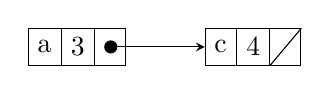
\begin{tikzpicture}[list/.style={rectangle split, rectangle split parts=3,draw, rectangle split horizontal}, >=stealth, start chain,baseline=-1mm]
\node[list,on chain] (A) {a \nodepart{second} $3$};
\node[list,on chain] (B) {c \nodepart{second} $4$};
\draw (B.two split south) -- (B.north east);
\draw[*->] let \p1 = (A.three), \p2 = (A.center) in (\x1,\y2) -- (B);
\end{tikzpicture}
,写成ML代码是\mintinline{sml}{("a",3)::("c",4)::nil}。

现在,令表$t_2$就像表$t_1$,不同的是,$c$映射到了$7$而不是$4$。我们可以将这个过程写为以下数学形式:

$t_2=update(t_1,c,7)$

其中函数update返回一个新表$\{a \mapsto 3,c \mapsto 7\}$。

在计算机中,只要我们假设在链表中$c$的\textit{第一次}出现优先于它较后的任何出现,就可以通过在表头插入一个新元素来实现新表$t_2$
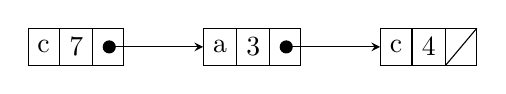
\begin{tikzpicture}[list/.style={rectangle split, rectangle split parts=3,draw, rectangle split horizontal}, >=stealth, start chain,baseline=-1mm]
\node[list,on chain] (C) {c \nodepart{second} $7$};
\node[list,on chain] (A) {a \nodepart{second} $3$};
\node[list,on chain] (B) {c \nodepart{second} $4$};
\draw (B.two split south) -- (B.north east);
\draw[*->] let \p1 = (A.three), \p2 = (A.center) in (\x1,\y2) -- (B);
\draw[*->] let \p1 = (C.three), \p2 = (C.center) in (\x1,\y2) -- (A);
\end{tikzpicture}
。

因此,update函数很容易实现,而与之相应的lookup函数

\begin{minted}{sml}
val lookup : table * id -> int
\end{minted}

则只要沿着链表从头向后搜索即可。

表达式的解释要比语句的解释复杂一些,因为表达式返回整型数值\textit{且}有副作用。我们希望解释器本身在模拟直线程序设计语言的赋值语句时不产生任何副作用(但是print语句将有解释器的副作用来实现)。实现它的方法是将interpExp的类型设计成exp $\times$ table $\rightarrow$ int $\times$ table。用表$t_1$解释表达式$e_1$的结果是得到一个整型数值$i$和一个新表$t_2$。当解释一个含有两个子表达式的表达式(例如OpExp)时,由第一个子表达式得到的表$t_2$可以继续用于处理第二个子表达式。

\section{习题}
\definecolor{myblue}{RGB}{60, 113, 183}

\begin{enumerate}
  \item 下面这个简单的程序实现了一种\textit{持久化}(persistent)函数式二叉搜索树,使得如果\mintinline{sml}{tree2 = insert(x, tree1)},则当使用tree2时,tree1仍然可以继续用于查找。
  \begin{minted}{sml}
    type key = string
    datatype tree = LEAF | TREE of tree * key * tree

    val empty = LEAF

    fun insert(key, LEAF) = TREE(LEAF, key, LEAF)
      | insert(key, TREE(l, k, r)) =
                    if key < k
                      then TREE(insert(key, l), k, r)
                    else if key > k
                      then TREE(l, k, insert(key, r))
                    else TREE(l, key, r)
  \end{minted}
  \begin{enumerate}
    \item 实现函数member,若查找到了相应项,返回true,否则返回false。
    \item 扩充这个程序使其不仅能判别成员关系,而且还能将键值
    \item 这个程序构造的树是不平衡的;用下述插入顺序说明树的形成过程:
    \begin{enumerate}
      \item t s p i p f b s t
      \item a b c d e f g h i
    \end{enumerate}
    \item [\textcolor{myblue}{(*d).}] 研究Sedgewick[1997]中讨论过的平衡搜索树,并为函数式符号表推荐一种平衡树数据结构。\textbf{提示:}为了保持函数式风格,算法应该在插入时而不是在查找时保持树的平衡,因此,不适合使用类似于\textit{伸展树}(splay tree)这样的数据结构。
  \end{enumerate}
\end{enumerate}

\chapter{词法分析}

\section{词法单词}

\section{正则表达式}

\section{有限自动机}

\section{非确定性有限自动机}

\subsection{将正则表达式转换为NFA}

\subsection{将NFA转换为DFA}

\section{ML-Lex:词法分析器的生成器}

\section{程序设计:词法分析}

\section{推荐阅读}

\section{习题}

\end{document}